\documentclass{beamer}
\usetheme{metropolis}
% \setbeamertemplate{navigation symbols}{} 

\AtBeginEnvironment{alltt}{\setlength{\topsep}{0pt}}

\titlegraphic{\hfill
\includegraphics[height=1cm]{figures/logo-dc.eps}}
\usepackage{textpos} 

\addtobeamertemplate{frametitle}{}{%
	\begin{textblock*}{0mm}(\textwidth-2cm,-1cm)
		
\includegraphics[height=1cm]{figures/logofondonegro.eps}
    \end{textblock*}
}
\setbeamertemplate{section in toc}[ball unnumbered] % index with bullet points
\setbeamercolor{block body}{bg=structure!10} % visible blocks
\setbeamercolor{block title}{bg=structure!20}
\setbeamertemplate{blocks}[rounded][shadow] %round the edges of the blocks and cast a shadow
%-------------------------------------------------------
\usepackage[spanish]{babel} % Para separar correctamente las palabras
\usepackage[utf8]{inputenc} % Este paquete permite poner acentos y eñes usando codificación
\usepackage[most]{tcolorbox}
\usepackage{wrapfig}
\usepackage{multimedia}

\usepackage{multicol}
\usepackage{listings}
\lstset{
    language=C,
    backgroundcolor=\color{black!5}, % set backgroundcolor
    basicstyle=\footnotesize,% basic font setting
}

\usepackage{trimclip}
%%%%%%%%%%%%%%%%%%%%%%%%%%%%%%%%%%%%%%%%%%%%%%%%%%%%%%%%%%%%%%%%%%%%%%%%%%%%%%%
%%  Modifiers and Fonts
%%%%%%%%%%%%%%%%%%%%%%%%%%%%%%%%%%%%%%%%%%%%%%%%%%%%%%%%%%%%%%%%%%%%%%%%%%%%%%%

\renewcommand{\k}[1]{\textit{#1}}
\newcommand{\mk}[1]{\mathit{#1}}

\renewcommand{\v}[1]{\texttt{#1}}
\newcommand{\mv}[1]{\text{\small\textsf{#1}}\xspace}
\newcommand{\mvs}[1]{\text{\scriptsize\textsf{#1}}\xspace}

\newcommand{\sref}[2]{\ref{#1}{\color{BrickRed}.}{\subref*{#1:#2}}}

%%%%%%%%%%%%%%%%%%%%%%%%%%%%%%%%%%%%%%%%%%%%%%%%%%%%%%%%%%%%%%%%%%%%%%%%%%%%%%%
%%  Symbols
%%%%%%%%%%%%%%%%%%%%%%%%%%%%%%%%%%%%%%%%%%%%%%%%%%%%%%%%%%%%%%%%%%%%%%%%%%%%%%%

% Tildes and crosses

\newcommand{\Y}{\ding{51}}
\newcommand{\N}{\ding{55}}

% Math

\newcommand{\card}[1]{\lvert#1\rvert}
\newcommand{\<}{\langle}
\renewcommand{\>}{\rangle}
\newcommand{\ldot}{\;.\;}
\newcommand{\lcom}{\,,\,}
\newcommand{\primeI}[1]{{#1}'}
\newcommand{\primeII}[1]{{#1}'\!\!\:'}
\newcommand{\into}{\mapsto}
\newcommand{\Nat}{\mathbb{N}}
\newcommand{\dotrightarrow}{\clipbox{0pt 0 {.675\width} 0}{\ensuremath{\rightarrow}} \makebox[1.1pt]{} {\cdot} {\cdot} {\cdot} \makebox[1.1pt]{} \clipbox{{.55\width} 0 0pt 0}{\ensuremath{\rightarrow}}}
\newcommand{\longdotrightarrow}{\clipbox{0pt 0 {.55\width} 0}{\ensuremath{\rightarrow}} \makebox[2pt]{} {\cdot} \makebox[1pt]{} {\cdot} \makebox[1pt]{} {\cdot} \makebox[2pt]{} \clipbox{{.45\width} 0 0pt 0}{\ensuremath{\rightarrow}}}

% Sets

\newcommand{\C}{\subseteq}
\newcommand{\x}{\times}

% Logic

\newcommand{\true}{\mk{true}}
\newcommand{\false}{\mk{false}}
\renewcommand{\iff}{\Leftrightarrow}
\newcommand{\then}{\Rightarrow}

% Tools

\newcommand{\MTSA}{{\scshape mtsa}\xspace}
\newcommand{\SUP}{{\scshape supremica}\xspace}
\newcommand{\MBP}{{\scshape mbp}\xspace}
\newcommand{\PRP}{{\scshape prp}\xspace}
\newcommand{\MYND}{{\scshape mynd}\xspace}
\newcommand{\RATSY}{{\scshape ratsy}\xspace}
\newcommand{\ACACIA}{{\scshape acacia+}\xspace}
\newcommand{\SLUGS}{{\scshape slugs}\xspace}
\newcommand{\CIRCA}{{\scshape circa}\xspace}
\newcommand{\PARTY}{{\scshape party}\xspace}
\newcommand{\GPT}{{\scshape gpt}\xspace}
\newcommand{\DCS}{{\scshape dcs}\xspace}

% Supervisory Control

\renewcommand{\l}{\ell}
\renewcommand{\ll}{{\bar{\l}}}
\renewcommand{\d}{\delta}
\newcommand{\init}[1]{\bar{#1}} % #1 state name
\newcommand{\state}[2]{{#1}^{#2}}
\newcommand{\s}[1]{\state{e}{#1}}

\newcommand{\D}{\rightarrow}
\newcommand{\B}{\rightsquigarrow}

\newcommand{\A}{\mathcal{A}}
\newcommand{\E}{\mathcal{E}}
\newcommand{\G}{\mathcal{G}}
\newcommand{\M}{\mathcal{M}}
\newcommand{\R}{\mathcal{R}}
\newcommand{\W}{\mathcal{W}}

\renewcommand{\L}{\mathcal{L}}
\renewcommand{\P}{\mathcal{P}}
\renewcommand{\S}{\mathcal{S}}

\newcommand{\w}{\ensuremath{\omega}}

\newcommand{\notstep}[2]{\overset{#1}{\not\D}_{#2}}
\newcommand{\step}[2]{\overset{#1}{\D}_{#2}}
\newcommand{\mstep}[2]{\overset{#1}{\twoheadrightarrow}_{#2}}
\newcommand{\lstep}[2]{\overset{#1}{\longrightarrow}_{#2}}
\newcommand{\walk}[2]{\overset{#1}{\Rightarrow}_{#2}}
\newcommand{\hop}[2]{\overset{#1}{\B}_{#2}}
\newcommand{\runw}[2]{\,\overset{#1}{\dotrightarrow}_{#2}\,}
\newcommand{\run}[3]{
\,\overset{#1\ldots#2}{\longdotrightarrow}_{#3}\,}
\newcommand{\runlst}[3]{
\overset{#1\quad#2}{\raisebox{.1pt}{-}{\,\cdot\cdot\cdot}\!\D}_{#3}}

\newcommand{\trimlst}[1]{\trimbox{0 0 0 5pt}{\ensuremath{#1}}}

% DCS

\newcommand{\ma}[1]{\tilde{#1}}
\renewcommand{\#}{\text{\rapprox}}
\newcommand{\rapprox}{\protect\raisebox{.09em}{\:\!\protect\reflectbox{\protect\rotatebox[origin=c]{90}{\ensuremath{\approx}}}}}

\newcommand{\dist}[1]{\makebox[6pt][c]{\raisebox{0pt}[6pt][1.5pt]{\ensuremath{\scriptscriptstyle #1}}}}

\newcommand{\CCC}{\mathbb{C}}
\newcommand{\WCCC}{\mathbb{W}}

\newcommand{\open}{\mk{open}}
\newcommand{\recommendations}{\mk{RT}} %{\mathcal{R}} %\mk{recommendations}
\newcommand{\Goals}{\mk{Goals}}
\newcommand{\Errors}{\mk{Errors}}
\newcommand{\NONE}{\mk{None}}
\newcommand{\Unsettled}{\mk{Unsettled}}
\newcommand{\Witness}{\mk{Witnesses}}

%nuevos:  ------------------------------------------------------------
\newcommand{\pathBetween}[2]{(#1 \step{\l}{E} #2\runw{}{\structure} #1)}

\newcommand{\unexploredToBottom}[1]{\mk{{#1}_{\bot}}}
\newcommand{\unexploredToTop}[1]{\mk{{#1}_{\top}}}

\newcommand{\cyan}[1]{\textcolor{cyan}{#1}}
\newcommand{\red}[1]{\textcolor{red}{#1}}

%\newcommand{\unexploredToBottom}[1]{\mk{#1_{?\rightarrow \bot}}}
%\newcommand{\unexploredToTop}[1]{\mk{#1_{?\rightarrow \top}}}

\newcommand{\forcedTo}[3]{\mk{(#1\twoheadrightarrow #2)_{#3}}}

\newcommand{\WES}{\mk{W_{\unexploredToBottom{\structure}}}}
\newcommand{\WESS}{\mk{W_{\unexploredToBottom{\structure'}}}}
\newcommand{\LES}{\mk{L_{\unexploredToTop{\structure}}}}
\newcommand{\LESS}{\mk{L_{\unexploredToTop{\structure'}}}}
\newcommand{\WE}{\mk{W_E}}
\newcommand{\LE}{\mk{L_E}}

\newcommand{\SCC}{\mk{loops}} %strongly connected component

\newcommand{\Loops}[2]{AllNoneLoops(#1,#2)}

%\newcommand{\controllerReachsGoalsInOneStep}[1]{\mk{(\exists \l \ldot \trimlst{#1 \step{\l}{E} e''} \wedge e'' \in \Goals)    \wedge (\forall \l_u \in A_E^U \ldot \trimlst{#1 \step{\l_u}{E} e''} \then e'' \in \Goals)}}


\newcommand{\marked}[2]{\mk{\exists e_m \in #1 \ldot e_m \in M_{#2}}}
\newcommand{\descendants}{\mk{descendants}}

\newcommand{\Targets}{Targets\newcommand{\Targets}{Targets}

}
%----------------------------------------------------------------------

\newcommand{\totalTests}{52}

\newcommand{\heuristic}{\mk{heuristic}}
\newcommand{\initial}{\ensuremath{\init{e}}}
\newcommand{\current}{\ensuremath{s}}
\newcommand{\child}{\ensuremath{s'}}
\newcommand{\structure}{\mk{ES}}
\newcommand{\toOpen}{\mk{toOpen}}

\newcommand{\ancestors}{\mk{ancestors}}
\newcommand{\predecesor}{\mk{predecesor}}
\newcommand{\statusu}{\mk{status}}
\newcommand{\visited}{\mk{visited}}
\newcommand{\pending}{\mk{pending}}
\newcommand{\unconfirmed}{\mk{unconfirmed}}

\newcommand{\target}{\mk{target}}
\newcommand{\novel}{\mk{novel}}
\newcommand{\distant}{\mk{distant}}
\newcommand{\strides}{\mk{strides}}

\newcommand{\MA}[2]{\mk{MA}_{#1}^{#2}}
\newcommand{\RA}[2]{\mk{RA}_{#1}^{#2}}

\newcommand{\g}{\ensuremath{g}}
\newcommand{\m}{m}%{\mathsf{m}}
\newcommand{\rr}{r}%{\mathsf{r}}
\newcommand{\pp}{p}%{\mathsf{p}}

%%%%%%%%%%%%%%%%%%%%%%%%%%%%%%%%%%%%%%%%%%%%%%%%%%%%%%%%%%%%%%%%%%%%%%%%%%%%%%%
%%  Environments
%%%%%%%%%%%%%%%%%%%%%%%%%%%%%%%%%%%%%%%%%%%%%%%%%%%%%%%%%%%%%%%%%%%%%%%%%%%%%%%

%\theoremstyle{break}
\newtheorem{theorem}{Teorema}
\newtheorem{proof}{Demostración Lemma}
\newtheorem{definition}{Definición}
\newtheorem{notation}{Notación}
\newtheorem{property}{Propiedad}
\newtheorem{lemma}{Lema}

%%%%%%%%%%%%%%%%%%%%%%%%%%%%%%%%%%%%%%%%%%%%%%%%%%%%%%%%%%%%%%%%%%%%%%%%%%%%%%%
%%  Spacing
%%%%%%%%%%%%%%%%%%%%%%%%%%%%%%%%%%%%%%%%%%%%%%%%%%%%%%%%%%%%%%%%%%%%%%%%%%%%%%%

%\newcommand{\merge}[2]{\multicolumn{#1}{c|}{#2}}

%\newcolumntype{L}[1]{>{\raggedright\let\newline\\\arraybackslash\hspace{0pt}}m{#1}}
%\newcolumntype{C}[1]{>{\centering\let\newline\\\arraybackslash\hspace{0pt}}m{#1}}
%\newcolumntype{R}[1]{>{\raggedleft\let\newline\\\arraybackslash\hspace{0pt}}m{#1}}
%\newcommand{\rb}[1]{\raisebox{-1.5pt}{#1}}


%%%%%%%%%%%%%%%%%%%%%%%%%%%%%%%%%%%%%%%%%%%%
\def\qed{\relax\ifmmode\hskip2em \Box\else\unskip\nobreak\hskip1em $\Box$\fi}


\newcommand<>{\reveal}[1]{\mbox{}\visible#2{#1}} % ej: \reveal<5->{text} aparece de 5 en adelante

\title[DCS non-blocking]{Directed Controller Synthesis for Non-Maximal Blocking Requirements}
\author[Duran, Zanollo]{Matias Duran, Florencia Zanollo}
\date[12/5/21]{12 de Mayo de 2021}
%-------------------------------------------------------
% INTRO
% intro sobre qué queremos (programa que soluciona problemas por nosotros)
% qué toma de input (autómatas, modelo de la realidad, en general son varios)
% detalles de los autómatas (estado inicial, marcados, etc) con ejemplo de avión
% la composición explota, los algor clásicos rompen acá (i.e. decir que existe algor monolítico)
% idea general: componer mientras exploras y terminar al tener conclusión (con suerte antes de ver todo)
% [buscar] ejemplo simple para explicar composición (mostrar planta completa)

% DEFINICIONES (ANTECEDENTES)
% def pasos y corridas
% controlador
% vemos en particular problemas non-blocking (i.e. loop para ganadores, no-controlables no joden)
% estados ganadores y perdedores (estados desde donde hay una estrategia==controlador ganadora/perdedora)

% ON-THE-FLY
% explicar exploración parcial (lo visto hasta ahora)
% estados ganadores y perdedores ahora (antes era facil, ahora tenemos que ver a dónde van)
% el concepto de ``frontera'' (en el sentido de transiciones existentes sin explorar) top, bottom
% actualizamos estado solo cuando estamos seguros (ganador en bottom / perdedor en top)
% exploramos de a una transición [e -l-> e']
% esto actualiza antecesores de e
% idea central de que ganador necesita loop

% TESTS
% implementación en MTSA, explicación mini de la herramienta
% hicimos tests, medio TDD

% BENCHMARK
% usamos mismo benchmark que dany
% resultados vs DCS version 1.0 y la nuestra (DCS2)

% QUÉ VIMOS (CONCLUSIONES)
% entender el problema
% soluciones existentes, idea nueva
% nuevo algoritmo, ``demo'' de corrección y completitud
% implementación
% batería de tests
% benchmark confirma que mantiene eficiencia
% esta idea se puede aplicar a otro tipo de problemas (que no sean non-blocking), ej GR1 vuelvan prontos
%-------------------------------------------------------
\begin{document}
%-------------------------------------------------------
\begin{frame}[plain]

\titlepage

\end{frame}
%-------------------------------------------------------
\begin{frame}[plain]{Índice}
    \tableofcontents
\end{frame}
%-------------------------------------------------------
\section{Introducción}% INTRO
% intro sobre qué queremos (programa que soluciona problemas por nosotros)
% qué toma de input (autómatas, modelo de la realidad, en general son varios)
% detalles de los autómatas (estado inicial, marcados, etc) con ejemplo de avión
% la composición explota, los algor clásicos rompen acá (i.e. decir que existe algor monolítico)
% idea general: componer mientras exploras y terminar al tener conclusión (con suerte antes de ver todo)
% [buscar] ejemplo simple para explicar composición (mostrar planta completa)
%-------------------------------------------------------
\begin{frame}{Objetivo}
    \begin{block}{}
    ``The good thing about computers is that they do what you tell them to do. The bad news is that they do what you tell them to do.''\hfill – Ted Nelson 
    \end{block}
    
    \pause
    ¿Es posible hacer que una computadora se diga a sí misma qué hacer?
    
    \pause
    \begin{block}{Síntesis Automática de Controladores}
     Se le brinda a un programa las reglas y objetivos a cumplir, éste sintetiza una estrategia para ganar (si existe) conocida con el nombre de controlador.
    \end{block}

\end{frame}
%-------------------------------------------------------
\begin{frame}{Control de Eventos Discretos}
    \begin{itemize}
     \item Es una de las áreas que estudia problemas de síntesis.
     \item El problema es modelado usando autómatas finitos (o máquinas de estados finitos).
     \pause
     \item Estos autómatas modelan la parte que nos interesa de la realidad.
     \item Se suele partir el modelo en pequeñas partes, más simples de abstraer, y luego se componen para formar el objeto de interés.
    \end{itemize}
\end{frame}
%-------------------------------------------------------
\begin{frame}{Autómatas} 
    [EJEMPLO DE AUTÓMATA]

    detalles de los autómatas finitos (estado inicial, marcados (ver si va), etc)
\end{frame}
%-------------------------------------------------------
\begin{frame}{Composición} 
    ejemplo simple para explicar composición (mostrar planta completa)
    explicar por arriba cómo se compone o cuál es la idea (la planta refleja el comportamiento del todo) (reglas para sincronización entre las partes)
\end{frame}
%-------------------------------------------------------
\begin{frame}{Explosión de estados}
    la composición explota [img de una planta gigante?], los algor clásicos rompen acá (i.e. decir que existe algor monolítico)
\end{frame}
%-------------------------------------------------------
\begin{frame}{Idea general de este trabajo}
    Partiendo de la versión presentada en la tesis doctoral de Daniel Ciolek, queremos componer mientras exploras y terminar al tener conclusión (con suerte antes de ver todo).
    
    Dicha versión presentaba errores a la hora de clasificar los estados, nuestra intención es, no sólo arreglar los errores, sino dar una demostración formal al respecto.
    
\end{frame}
%-------------------------------------------------------

%-------------------------------------------------------
\section{Conocimiento previo}% DEFINICIONES (ANTECEDENTES)
% def pasos y corridas
% controlador
% vemos en particular problemas non-blocking (i.e. loop para ganadores, no-controlables no joden)
% estados ganadores y perdedores (estados desde donde hay una estrategia==controlador ganadora/perdedora)
%-------------------------------------------------------
\begin{frame}{Acciones, pasos y corridas (run)}
    \begin{figure}
        \begin{overprint}
        \onslide<1>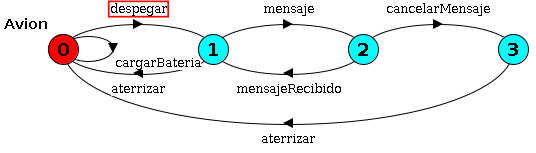
\includegraphics[width=\textwidth]{figures/1accion.png} 
        \onslide<2>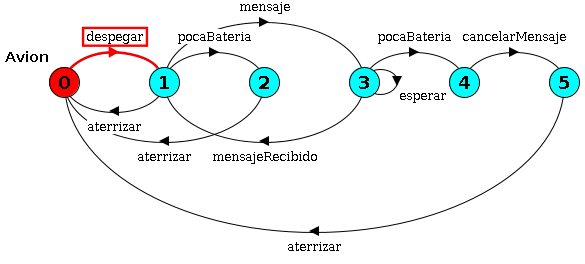
\includegraphics[width=\textwidth]{figures/2paso.png} 
        \onslide<3->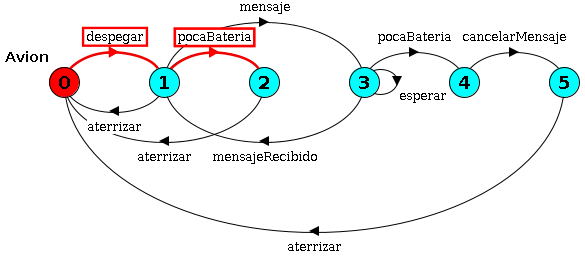
\includegraphics[width=\textwidth]{figures/3run.png} 
        \end{overprint}
    \end{figure}

    \begin{itemize}
     \item Acción es una transición entre los estados.
     \pause
     \item Un paso es $t \step{\l}{T} t'$, toma en cuenta el estado de partida y llegada.
     \pause
     \item Una corrida de una palabra $w = \l_0,\ldots,\l_k$ en $T$, es $t_0 \runw{w}{T} t_{k+1}$, es decir, varios pasos.
    \end{itemize}
    
\end{frame}
%-------------------------------------------------------
\begin{frame}{Problema de control non-blocking}
    \begin{block}{¿Cuál es la entrada de un problema de control?}
        \begin{itemize}
          \item conjunto de autómatas (la composición de ellos es la planta completa que no queremos calcular)
          \item acciones controlables y no controlables
          \item estados marcados u objetivos (se quiere tener la \textit{posibilidad} de visitar infinitas veces \textit{al menos uno})
        \end{itemize}
    \end{block}

    \begin{block}{¿Qué devuelve?}
        Una estrategia ganadora (llamada controlador) o afirmación de que no existe.
    \end{block}

\end{frame}
%-------------------------------------------------------
\begin{frame}{En nuestro ejemplo}
    \begin{description}
     \item[Conjunto de autómatas] Avión, Batería.
     \item[Acciones controlables] despegar, aterrizar, mensaje, cargarBateria, cancelarMensaje.
     \item[Acciones no-controlables] mensajeRecibido, pocaBateria.
     \item[Objetivo] Enviar \textit{mensaje}.
    \end{description}
    
    \textbf{Planta} (composición de todos los autómatas)
    \begin{figure}
     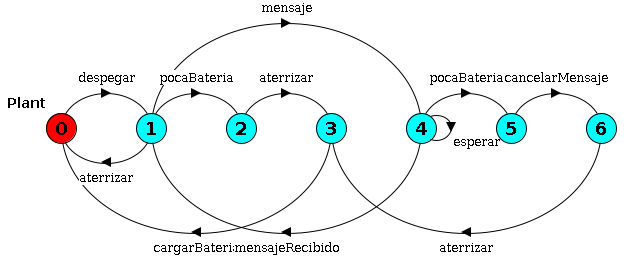
\includegraphics[width=\textwidth]{figures/planta.png}
    \end{figure}
    
\end{frame}
%-------------------------------------------------------
\begin{frame}{Controlador}
    \begin{figure}
     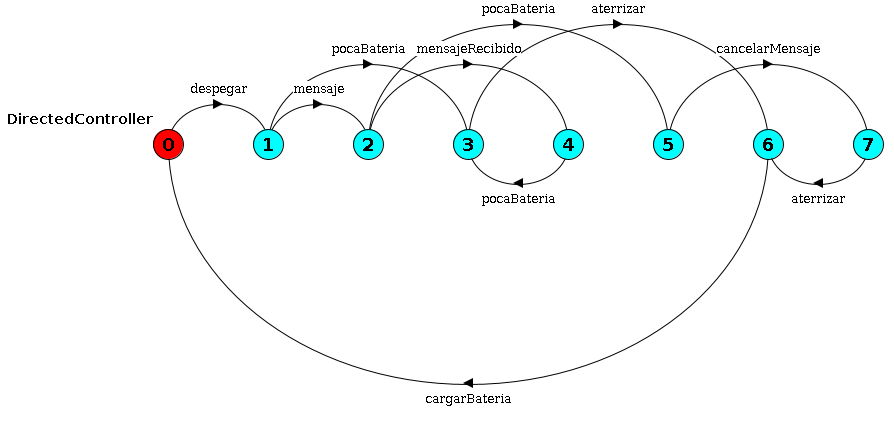
\includegraphics[width=\textwidth]{figures/director.png}
    \end{figure}

    Es una restricción de la planta que cumple las reglas:

    \begin{itemize}
     \item Puede prohibir pasos controlables.
     \item Mantiene todas las acciones no-controlables.
     \item Todas las corridas posibles en la planta restringida pasan por algún estado marcado.
    \end{itemize}
\end{frame}
%-------------------------------------------------------
\begin{frame}{Estados ganadores y perdedores}
	
	\begin{wrapfigure}{r}{0.48\textwidth}
		\vspace{-1cm}
		\hspace{-0.8cm}
		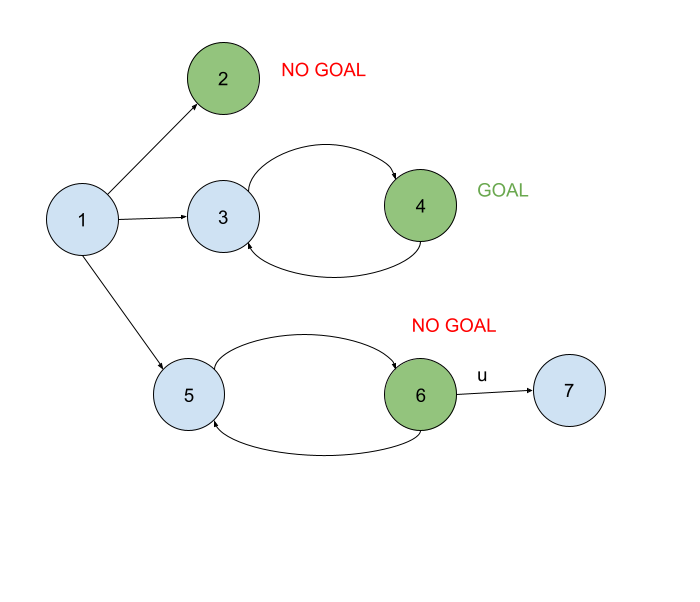
\includegraphics[width=0.6\textwidth]{figures/como-marcar-goals-FACAS.png}
	\end{wrapfigure}
	
    Si existe un controlador comenzando desde un estado, es decir, existe estrategia ganadora a partir del estado, entonces lo consideramos estado ganador. 
    Caso contrario, el estado es perdedor y debemos evitarlo.
    
    \vspace{0.5cm}
    \begin{block}{Observación}
        En particular nos interesa mucho si el estado inicial es ganador/perdedor, ya que eso nos dice si existe o no un controlador \textit{empezando} desde ahí.
    \end{block}

\end{frame}
%-------------------------------------------------------

%-------------------------------------------------------
\section{On-the-fly}% ON-THE-FLY
% explicar exploración parcial (lo visto hasta ahora)
% estados ganadores y perdedores ahora (antes era fácil, ahora tenemos que ver a dónde van)
% el concepto de ``frontera'' (en el sentido de transiciones existentes sin explorar) top, bottom
% actualizamos estado solo cuando estamos seguros (ganador en bottom / perdedor en top)
% exploramos de a una transición [e -l-> e']
% esto actualiza antecesores de e
% idea central de que ganador necesita loop


%dividimos en dos la explicación on-the-fly
%-------------------------------------------------------
\begin{frame}{Exploración parcial}
    La idea es intentar sacar conclusiones a medida que se explora, y construye a la vez, la composición total.
    
    Por ejemplo, en un momento dado podríamos tener explorado lo siguiente:
    \begin{figure}
     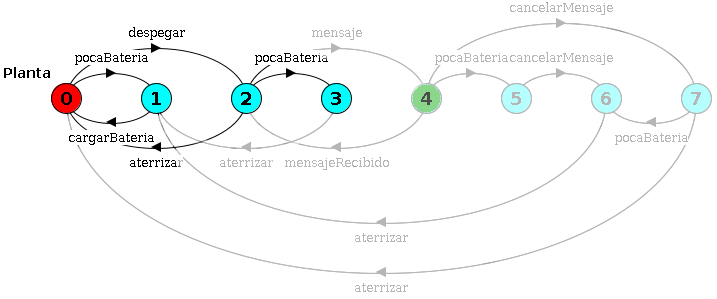
\includegraphics[width=\textwidth]{figures/partial.png}
    \end{figure}
    
    Exploramos de a una transición $e \step{\l}{} e'$ o paso.\vspace{10pt}\footnote{Los llamamos $e$ en vez de $t$ para resaltar que son \textit{estados de la planta}}
\end{frame}
%-------------------------------------------------------
\begin{frame}{Frontera optimista y pesimista}
    \begin{figure}
     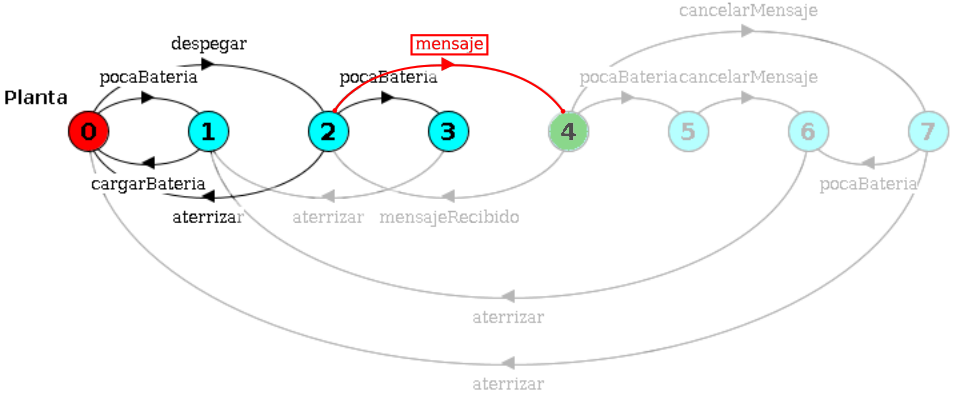
\includegraphics[width=\textwidth]{figures/frontera.png}
    \end{figure}
    El paso $2 \step{mensaje}{} 4$ está sin explorar. Como en principio no sabemos nada de él podríamos pensar que nos lleva a un estado ganador (frontera optimista) o perdedor (frontera pesimista).
\end{frame}
%-------------------------------------------------------
\begin{frame}{Nueva definición de ganadores/perdedores}
    Antes era simple reconocer ganadores/perdedores porque contábamos con toda la información de la planta; ahora debemos ``imaginar'' a dónde van a parar las transiciones no vistas.
    
    Actualizamos estados sólo cuando estamos seguros, es decir, señalamos ganadores sólo al pensar una frontera pesimista y perdedores en frontera optimista.
    
    \begin{block}{Observación}
        Los estados ganadores/perdedores según esta definición son ganadores/perdedores en la planta completa, es decir, una vez que clasificamos un estado nunca debemos reconsiderarlo.
    \end{block}
\end{frame}
%------------------------------------------------------- %parte 2
\begin{frame}{Propagar información}
    Lema2 ganador/perdedor es antecesor explicar por qué o lema o ej de imágen, ver la mejor manera\\
    Lema3 hay info para propagar si e' era conocido Y era gandor/perdedor (cc. no sabemos nada nuevo)
\end{frame}
%-------------------------------------------------------
\begin{frame}{Obtener nueva información (Ganador)}
    Lema4 explicar que necesitamos un loop para ganar, entonces sólo va a haber ganadores nuevos al encontrarnos dicho loop (i.e. el e' es uno que vimos Y no es ni ganador/perdedor porque sino cae en el caso anterior)
\end{frame}
%-------------------------------------------------------
\begin{frame}{Obtener nueva información (Perdedor)}
    Lema5 si ya exploraste todo y no hay marcados por ningún lado entonces obvio que no podés llegar a ninguno [dibujo]
\end{frame}
%-------------------------------------------------------
\begin{frame}{Resúmen del nuevo algoritmo}
    \begin{itemize}
     \item Clasificamos (ganador/perdedor) cuando estamos seguros. %i.e. no se cambia una vez que está
     \item Propagamos a los antecesores afectados (si hay información respecto a e').
     \item Tratamos de obtener nueva información sólo al cerrar loops.
    \end{itemize}
    
    \begin{block}{Observación:}
        Sólo hacemos nuevos cálculos cuando son realmente necesarios.
    \end{block}
    
    Nos interesa saber qué tan buena es la eficiencia del algoritmo, en tiempo de cómputo.
\end{frame}



%-------------------------------------------------------
\section{Implementación y Tests}% TESTS
% implementación en MTSA, explicación mini de la herramienta
% hicimos tests, medio TDD
%-------------------------------------------------------
\begin{frame}{Herramienta MTSA}
    \begin{itemize}
    	\item El LaFHIS, donde hicimos esta tesis, trabaja hace años en MTSA, una herramienta propia para resolver problemas de control con LTS.
    	\item Implementamos el algoritmo en java, agregándolo a las capacidades de MTSA. Esto permitió ejecutar los tests y el benchmark de la próxima sección.
    \end{itemize}
\end{frame}
%-------------------------------------------------------
\begin{frame}{Test Driven Development}
	\begin{itemize}
		\item Para ganar seguridad en nuestro código, y encontrar errores, fuimos armando una batería de tests.
		\item Con cada error encontrado en la implementación o la especificación del algoritmo, armábamos un nuevo test que detectara ese error, y luego lo arreglábamos.
		\item Quedaron 49 tests pequeños diseñados a mano para correr rápido y presentar las condiciones más problemáticas para nuestro algoritmo.
		\item Ésta batería de tests fue añadida a las utilizadas por la herramienta como tests de regresión para alertar problemas por futuros cambios en el código.
	\end{itemize}
\end{frame}
%-------------------------------------------------------
\begin{frame}{Ejemplo de MTSA en uso}
	\begin{figure}
		\hspace{-2cm}
		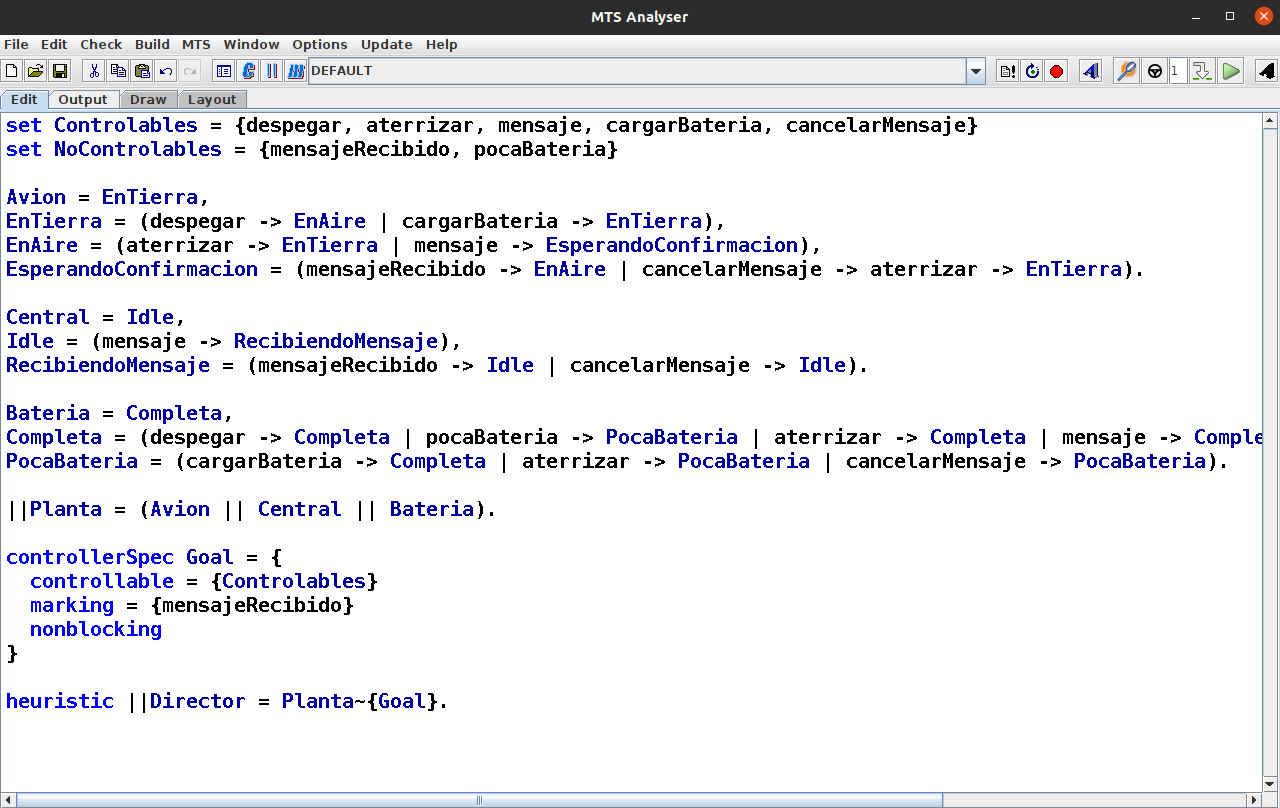
\includegraphics[width=\textwidth]{figures/HPWindow-ej.png}
	\end{figure}
	\pause
	\begin{picture}(0,0)
		\put(70,-10){
			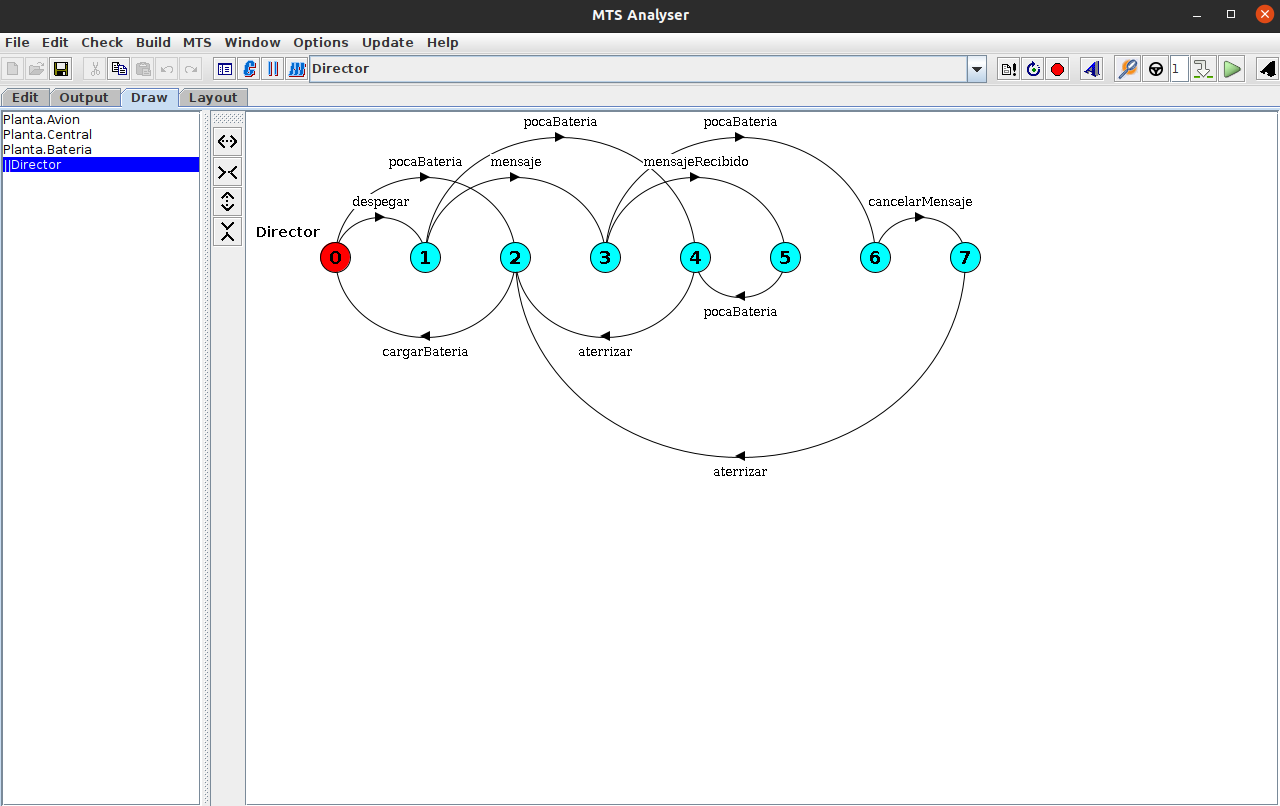
\includegraphics[width=\textwidth]{figures/controller-drawing-ej.png}
		}
	\end{picture}
\end{frame}
%-------------------------------------------------------
\begin{frame}{Animando controladores}
	Video de controlador animado?
\end{frame}
%-------------------------------------------------------

%-------------------------------------------------------
\section{Benchmark}\begin{frame}{Benchmark}
    \begin{itemize}
     \item Para realizar las pruebas de performance usamos el mismo conjunto de problemas utilizado para medir la versión anterior del algoritmo de exploración, recompilados por Daniel Ciolek en su tesis doctoral.
     
     \item Es un conjunto de seis tipos de problemas bastante clásicos, cada uno con dos partes parametrizables (n, k), en función de observar hasta qué tamaño de problema (n*k) soporta el algoritmo.
     
     \item DCS y DCS2 representan la versión anterior/nueva del algoritmo respectivamente.
     
     \item Utilizamos distintas estrategias a la hora de explorar, algunas más complejas (MA, RA) desarrolladas por Ciolek y una simple (BFS). La última fue agregada para obtener una idea de cuánto se puede mejorar cambiando la forma de explorar.
    \end{itemize}

\end{frame}
%-------------------------------------------------------
\begin{frame}{Performance (TL, DP, CM)}
    \begin{figure}
        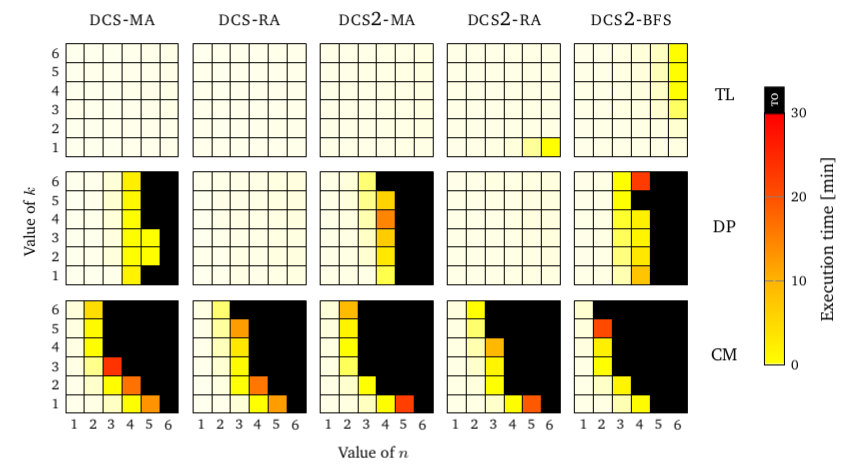
\includegraphics[width=\textwidth]{figures/benchmark1.png}
    \end{figure}

    Transfer Line, Dinning Philosophers, Cat and Mouse
    
\end{frame}
%-------------------------------------------------------
\begin{frame}{Performance (AT, BW, TA)}
    \begin{figure}
        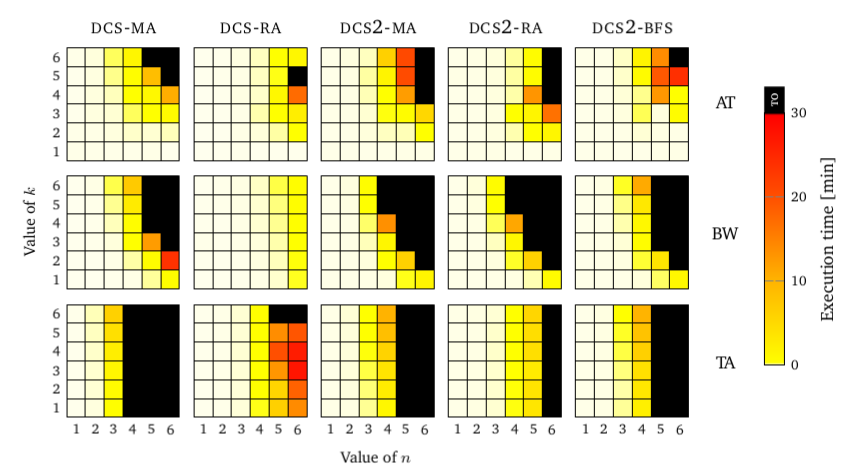
\includegraphics[width=\textwidth]{figures/benchmark2.png}
    \end{figure}

    Air-Traffic Management, Bidding Workflow, Travel Agency
\end{frame}

%-------------------------------------------------------
\section{Conclusión}
\begin{frame}[plain]{Qué vimos}
    \begin{itemize}[<+->]
    \item Definición del problema
    \item Soluciones existentes y la idea ``nueva'' (exploración on-the-fly)
    \item Nuevo algoritmo, parte de su demostración (corrección y completitud)
    \item Implementación en MTSA
    \item Batería de tests, TDD
    \item Benchmark y resultados versus la versión anterior. No se perdió eficiencia, teniendo en cuenta la confianza ganada en correctitud. En la tesis se encuentran además resultados de benchmark versus otras herramientas del estado del arte.
    \end{itemize}

    \begin{block}<7->{}
    La idea de exploración on-the-fly, y gran parte de la estructura del algoritmo, se puede aplicar a otro tipo de problemas, ej: GR1 (próximamente).
    \end{block}
\end{frame}
%-------------------------------------------------------
\begin{frame}[plain]{\null} % el null esta para forzar el header, alto trucazo
    \begin{columns}
    \begin{column}{0.5\textwidth}
        \Huge ¿Preguntas?\\
        
        \normalsize Gracias, vuelvan prontos\\ 
        \scriptsize (para ver GR1)
    \end{column}
    \begin{column}{0.5\textwidth}
        
\includegraphics[scale=0.5]{figures/apu.png}
    \end{column}
    \end{columns}
\end{frame}
%-------------------------------------------------------
\begin{frame}{Bonus track: Detalles de la exploración}    
    \begin{columns}
    \begin{column}{0.8\textwidth}
        \begin{figure}
        \centering
            \begin{overprint}
                \onslide<1>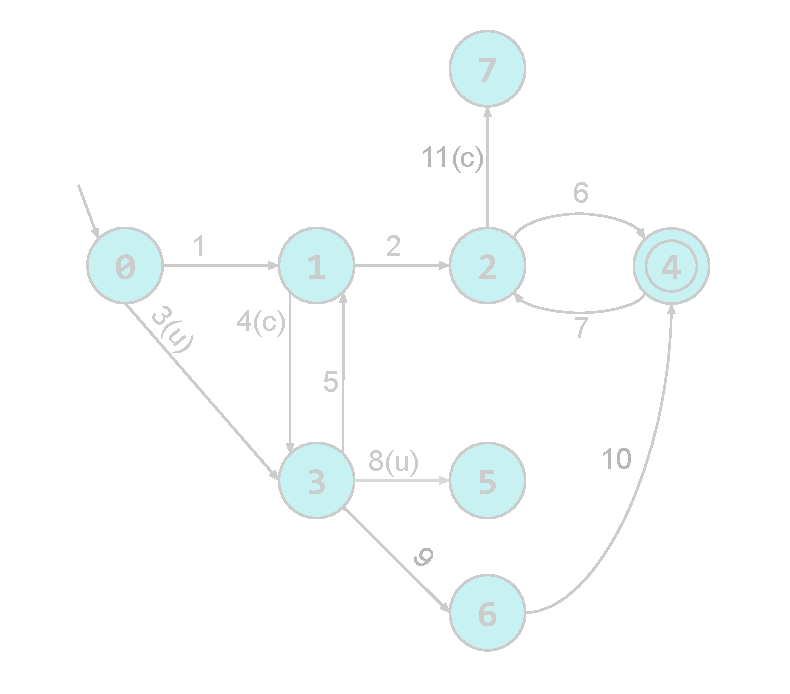
\includegraphics[scale=0.55]{../figures/ejemplo_on-the-fly/5.pdf}
                \onslide<2>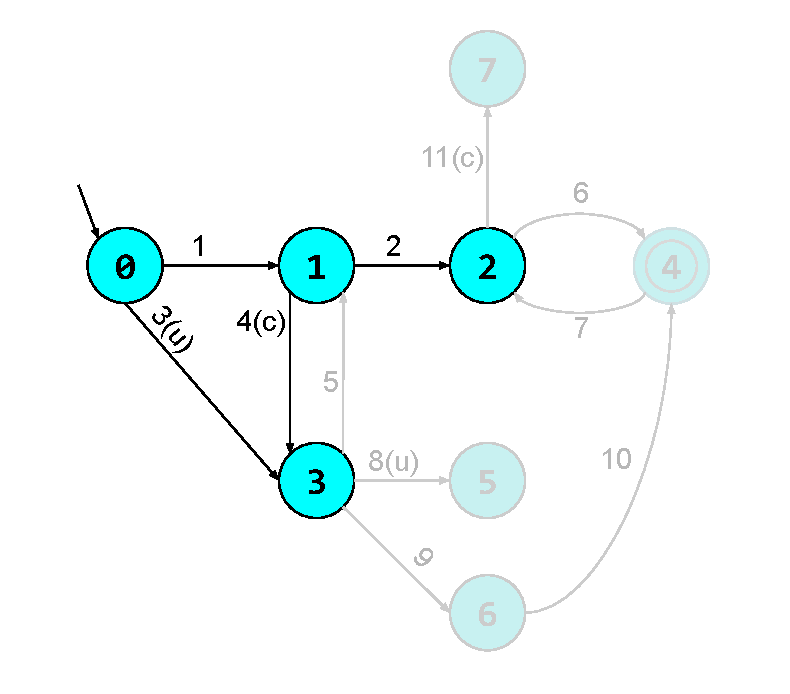
\includegraphics[scale=0.55]{../figures/ejemplo_on-the-fly/1.pdf}
                \onslide<3>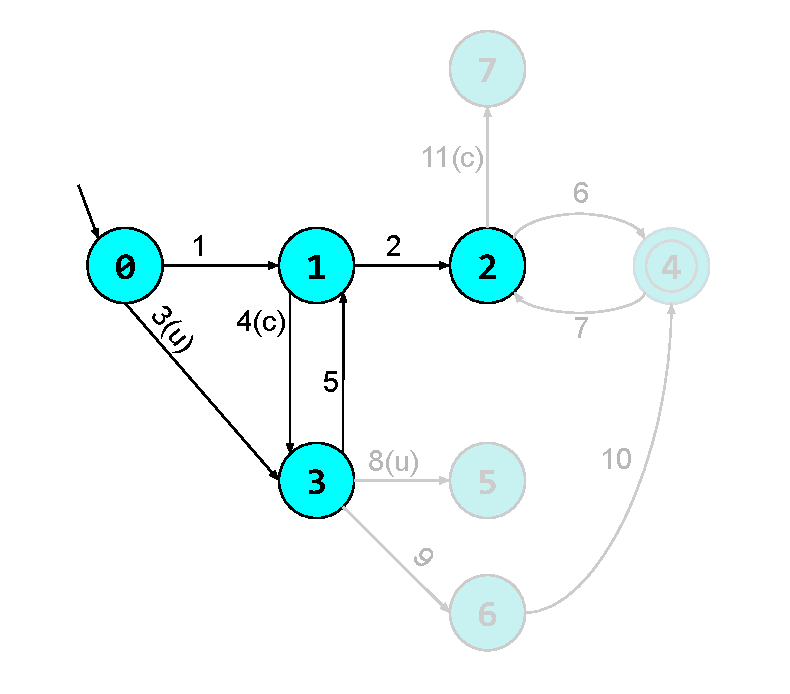
\includegraphics[scale=0.55]{../figures/ejemplo_on-the-fly/2.pdf}
                \onslide<4>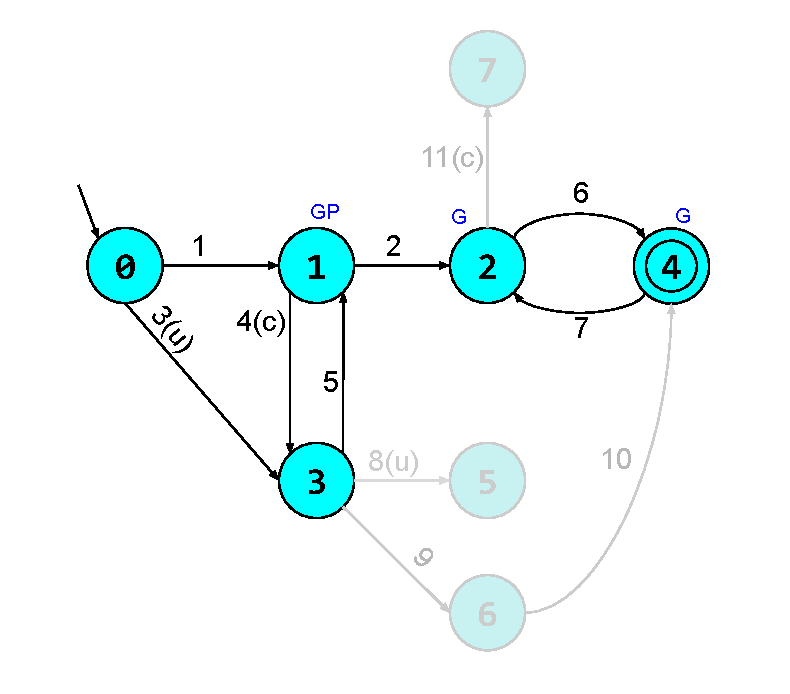
\includegraphics[scale=0.55]{../figures/ejemplo_on-the-fly/3.pdf}
                \onslide<5->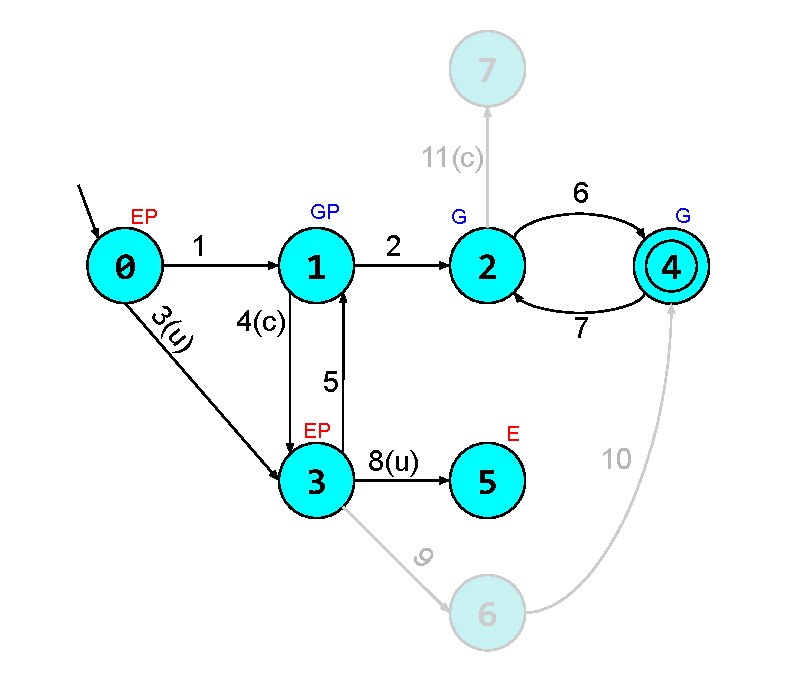
\includegraphics[scale=0.55]{../figures/ejemplo_on-the-fly/4.pdf}
            \end{overprint}
        \end{figure}
    \end{column}
    \begin{column}{0.4\textwidth}
        \hspace{-50pt}
        \begin{overprint}
            \onslide<2>Empieza por el estado \textbf{0} y mira los pasos:
                \begin{itemize}
                 \item $0 \step{1}{} 1$
                 \item $1 \step{2}{} 2$
                 \item $0 \step{3(u)}{} 3$
                 \item $1 \step{4(c)}{} 3$
                \end{itemize}

            \onslide<3>Explora el paso $3 \step{5}{} 1$\\
            Cierra loop pero todavía no hay estado marcado (u objetivo).
                 
            \onslide<4>Mira los pasos:
                \begin{itemize}
                 \item $2 \step{6}{} 4$
                 \item $4 \step{7}{} 2$
                \end{itemize}
                Cierra loop que incluye el estado marcado \textbf{4}, encontramos una parte ganadora, propagamos esa información.
                
            \onslide<5->Explora $3 \step{8}{} 5$, encuentra que \textbf{5} es perdedor y propaga la información. Llega al inicial entonces concluye que no hay controlador.
        \end{overprint}
    \end{column}
    \end{columns}

\end{frame}
%-------------------------------------------------------
\end{document}
